\documentclass{report}
\usepackage[utf8]{inputenc}
\usepackage{times}
\usepackage{cite}
\usepackage{hyperref}
\usepackage{tablefootnote}

\hypersetup{
    colorlinks,
    citecolor=black,
    filecolor=black,
    linkcolor=black,
    urlcolor=black
}
\begin{document}

\title{Distributed Audio Processing}
\author{Alexander Gustafson\\
  University of Applied Sciences,\\
  Zürich,\\
  Switzerland,\\
  alex\_gustafson@yahoo.de}
\date{\today}
\maketitle

\chapter*{Abstract}
In modern profesional music studios, the computer has become responsible for tasks that were previously performed by dedicated equipement. Mixing boards, effect processors, dynamic compressors and equalizers, even the instruments themselves, are all available as software. To elivate the processing load on the CPU there is a growing market for specialized DSP coprocessors which can process mutliple channels of digital audio in realtime. These coprocessors are typically connected via Firewire or PCIe and use multiple DSP chips for the processing. This project will examine an inexpensive alternative based on standard Gigabit Ethernet and higher end Raspberry Pi clones.



\chapter*{Declaration}
I declare that..

\tableofcontents

\chapter{Introduction}
\section{Ausgangslage}

20 years ago the CPU was just one component of a typical music studio. It was generally used to control and synchronize other equipement such as mixing boards, multitrack recorders, synthsizers and
effects processors. Today all of the other equipement exists as software, running in realtime on a CPU host. A typical music studio today is comprised of a CPU, multiple analog to digital inputs and outputs, and some DSP equiped audio processing cards. 

Simliar to GPU Cards which can accelerate graphics and visualization applications, audio DSP cards can process multiple streams of high qualtiy digital audio, eliviating the load on the CPU Host Computer. Audio DSP cards typically connect to the CPU via PCI, Firewire, or Thunderbolt. Most vendors of DSP cards offer the possibility to connect several cards in parallel to increase the processing capacity.

Unlike GPU processors however, no standard similar to OpenGL has develped which allows software from one vendor to run on hardware from another. Also, unlike OpenGL applications, audio software that is developed to run on an audio DSP card cannot be run on the CPU host. This results in vendor lock-in,
the consumer that invests in an audio DSP card and software, must continue to buy from the same vendor in order to build on the the initial investment. If another vendor of DSP hardware creates a superior product, a consumer is unlikely to switch platforms if a significant investment has already been made.  

10 years ago this was an acceptable compromise because DSP processors connected via PCIe could provide a significant performance increase. Today however, arm based inexpensive CPUs connected via standard gigabit ethernet could offer a competative alternatvie. 

\section{Ziel der Arbeit}


\chapter{Glossary}

\subsection*{MIDI}
The Musical Instrument Digital Interface specification, first introduced in 1983 defines an 8-bit standard for encoding and transmitting music notes. It's original purpose was to allow one keyboard based synthesizer to controll other music devices.\cite{Boulanger:2011} Allthough the specification also describes the hardware and wiring for daisy chaining instruments in a midi "network" most midi communication today transmitted via usb or virtually between audio software.

\subsection*{Zeroconf}
Zeroconf is a network service discovery protocl. It is also known as Bonjour, and occasionally refered to as Rendezvous, from the Apple implementations. Howl and Avahi are alternative open source Zeroconf implementations for Linux. Application can use Zeroconf to register or browse for service on a network without the need for a user to provide a specific IP Adress or port number. \cite{zeroconf}

\subsection*{AES67}

\subsection*{Latency}

\subsection*{VST}
\subsection*{SBC}
\subsection*{AVB}

\chapter{Einführung ins Thema}
\section{Background}

An audio engineer's typical job is to manage the balance of multiple tracks of audio signals. The dynamic range of a signal can be compressed, in order to give quiter passages more presence. Loud peaks can be limited to balance the overall loudness of a musical piece. Using equalizers an audio engineer can make enhance or supress specific frequencies of a track to make it more present in a mix. Effects like reverb, echo, or chorus can be used to give a track more space in a mix effecting the mood or ambience of a music piece. It is typcial that each track in a recording session will be processed by a chain of several specific audio processors.

20 years ago the equipment needed for this kind of processing filled large racks. Today all of these tasks run as plugins on the CPU.

In 1996 Steinberg GmbH, the developers of Cubase, a popular audio production application, released the VST interface specification and SDK.\cite{VST-wikipedia} The VST plugin standard was special because it allowed realtime processing of audio in the CPU and it allowed other developers to programm plugins which could be run from within Cubase. The VST plugin standard quickly had widespread industry acceptance and was adopted by most developers of audio production applications. Although alternative standards exist, VST is still the most widely adopted crossplatform standard.

The number of realtime plugins that could run on a CPU was limited by several factors, hard disc access speeds, bus speeds, amount of ram, and OS schedulers for instance\cite{brandt1998low}. User's didn't expect to be able to run more than 10 plugin instances at a time. Simply playing back multiple tracks of digital audio in realtime was so taxinig on the CPU that an application's graphical interface would quickly become unresponsive.

Today it's possible to playback hundreds of channels of audio and hundreds of plugins in realtime. But as the performance threshhold has risen, so to have the expectations. The algorithms driving today's plugins are much more complex that those from 1996. Plugins are available today that model physical systems or emulate the analog circutry of popular vintage synthsizers. So, even though CPU performance has increased significantly, it's still easy to reach the limits, especially with the more complex high qualtiy plugins.

Serval DSP based systems exist that can alleviate the load on the CPU much in the same way that GPU accelerator cards work. Audio processing jobs are delegated to external specialized hardware via PCIe or Thunderbolt interfaces. However, these DSP based accelerators are proprietary and expensive. Developing plugins for a DSP chip is also significatly more complex than developing for the CPU.


\section{Realtime Audio Plugins}

Music composition and production is typically done with the assistance of a music sequencing application. Midi events and audio recordings are arranged as tracks that can be mixed, edited, and processed. In order to make changes undo-able edits are made in a non-destructive fasion, calculated dynamically in realtime during audio playback. The original audio data is always preserved. The user can change the parameters of an effect or process in realtime and experiment with various parameters without fearing that the original audio recording might be permenantly altered.

A music sequencer or audio production application will usually include several built in realtime effects that a user can apply to an audio track. In addition to the built in options all professional applications will also be able to load 3d party effect plugins. Depending on the platform and vendor one or several available plugin standard will be implmeneted, the most common standard being Steinberg's VST standard.

Regardless of the standard most audio plugins function in a similar fashion. The host application will periodically poll the plugin via a callback, providing access to the source audio data stream and expecting the plugin to return the processed data.

Audio plugins can also provide a gui to the user that allows processing parameters to be modified, saved, and sequenced as well. This might be the cutoff frequency of a low pass filter, or the delay time of a reverb effect, for example.

On the Windows platform VST plugins are compiled to Dynamic Link Libraries, on Mac OSX they are Mach-O Bundles. The native apple Audio Unit plugins are also compiled as Mach-O bundles, they have almost identical functionality, but differ in their API implementation. Other alternative plugin formats are Avid's RTAS and AAX plugin formats, Microsoft's DirectX architecture, or LADSPA, DSSI and LV2 on Linux. From a programmer's point of view audio plugins are always compiled as dynamically loadable libraries that stricly conform to a format's specific API. The host application can load then at run time and stream audio data through them\cite{realtime-architectures}.

Additionally Realtime Audio Plugins, as the name implies, must be able to complete thier tasks fast enough to comply with realtime audio requirements. How fast is fast enough? Well, that depends how you define "real time". In audio applications, real time is defined in terms of an audio system's latency. The total delay between the time an audio signal enters the system (at the analog to digital converter for example), is processed, and leaves the system (at the digital to analog conterver) is the latency. If a musician is performing live and simultaneously hearing the result of the performance after being processed digitally, the system's latency must be low enough to feel instantaneous. The maximum acceptable latency is considered to be around 10ms\cite{AES67-2013}. Any higher and the latency becomes disturbing and not acceptable for live performance applications.

Any process will introduce some ammount of delay. Some processes, like those that rely on an FFT for example, need to work on a group of samples, introducing additional latency. Within the audio processing function, the programmer must take care not to introduce any unneccessary or uncalculateable delays. Examples for things to avoid are memory allocations, conditional expressions inside loops that might break pipe-lining optimizations\cite{realtime-architectures}, or updating the graphic interface directly.


\section{Audio Over Ethernet}

Sending audio data over a network is not new. Sending audio data in "realtime" is also not new. The IETF ( Internet Engineering Task Force ) RFC 3550 Describes the Real-time Transport Protocol for delivering audio and video in real-time over IP networks. RTP however is mostly concerned with transmitting a few channels of media as quickly as possible over IP networks with lot of other traffic, reducing jitter (variations in latency) and providing Quality of Service strategies to achieve "acceptable" audio and video quality for streaming and conferencing purposes.

Other specifications such as AVB\footnote{Audio Video Bridging refers to a set of IEEE standards that allow time-synchronized low latency streaming services } and AES67\footnote{AES67, created by the Audio Engineering Society, defines standard that allow existing low latency streaming systems to interoperate. AES67 does not define any new technologies but attempts to set a lowest common denominator by which existing standards can be compatible. } build on top of RTP and add more mechanisms to guarentee acurate timing and synchronization across a network for professional audio applications. The synchronisation is important in these applications because they are concerned with driving audio hardware attached to different hosts on a network.

Hardware synchronization and jitter management are not relevent to this project because we are not concerned with external audio hardware. The goal of this project it to utilise external cpus as audio coprocessors. Even so, the AVB and AES67 standards offer many insights into how to optimize data transmissionfor low latency applications and they also offer a proof-of-concept that it must be possible. The AES67 Specification's recomended packet times offer latencies well below 1 ms for hundred of simultaneos channels of high quality audio. This is well above legacy PCI and Firewire rates used for DSP based coprocessing\cite{bouillot2009aes}.

\section{Single Board Computers}

The popularity of the Raspberry Pi has spurned a whole industry around single-board computers (SBCs). Based on hardware used in mobile phones, these small low power devices are extremely popular because they are inexpensive and easy to use. The biggest advantage of SBCs compared to other embeded devices ist that they can run the Android and Linux operating systems, allowing them to be programmed using the same tools available on desktop computers.

Recent higher-end SBCs even come equiped with gigabit Ethernet and Dual and Quad Core CPUs running at rates well over 1GHz. If we compare these systems to the 450MHz G3 PPC systems that the first VST Software was available for we can expect that the newer high-end SBCs should be excellent audio coprocessors.

2 SBCs are worth special consideration because they potentially offer even better performance as audio coprocessors. The Parallella Board has a 16-Core Epiphany co-processor that could be used to perform audio processing in parallel. Standard frameworks such as OpenCL, MPI, or OpenMP can be used to target the Epiphany cores. The Odroid-XU4 SBC includes a Mali-T628 GPU coprocessor which is also OpenCL compatible. Both are available for under \$100.

Programming audio processing routines as OpenCL kernals might be considerably more complex than in C++, but OpenCL offers vendor-independent access to GPGPU computing and has the added benefit that it can also be used on a CPU without GPU acceleration\cite{vst-gpu}.

Investigating these, and other OpenCL enabled SBCs might be an interesting followup project.
\section{Virtual Analog Synthesis}

Virtual analog synthesis is the term used to describe the emulation of analog synthsizers of the 60s and 70s digitally in real time. The complexity and goals of an emulation can vary. Some emulations go so far as to simulate the actual electronic components of vintage synthesis circuits, others just model ths signal flow loosly.

Regardless of the type of emulation, and model of analog systhesis has two primary concerns. Latency and aliasing. The problem of latency has already been described above. Any processing will introduce a delay in the signal, the complexity of the processing can increase the delay, or use more CPU cycles. Aliasing is audible distortion introduced by signals that have a higher frequency content than the sampling rate of the system allows for.

Analog synthsizers usually employed what is refered to as subtractive synthsis. One or more sound generators or oscillators would create signals with particular harmonic qualities. These signals would then go through filters that would "subtract" frequencies from the signal. The oscillators and filters can be modulated as well as the amplitude of the filtered signal. Figure~\ref{fig:synth_voice_block} is a simple block diagram of a typical subtractive synth voice.

\begin{figure}[H]
    \centering
    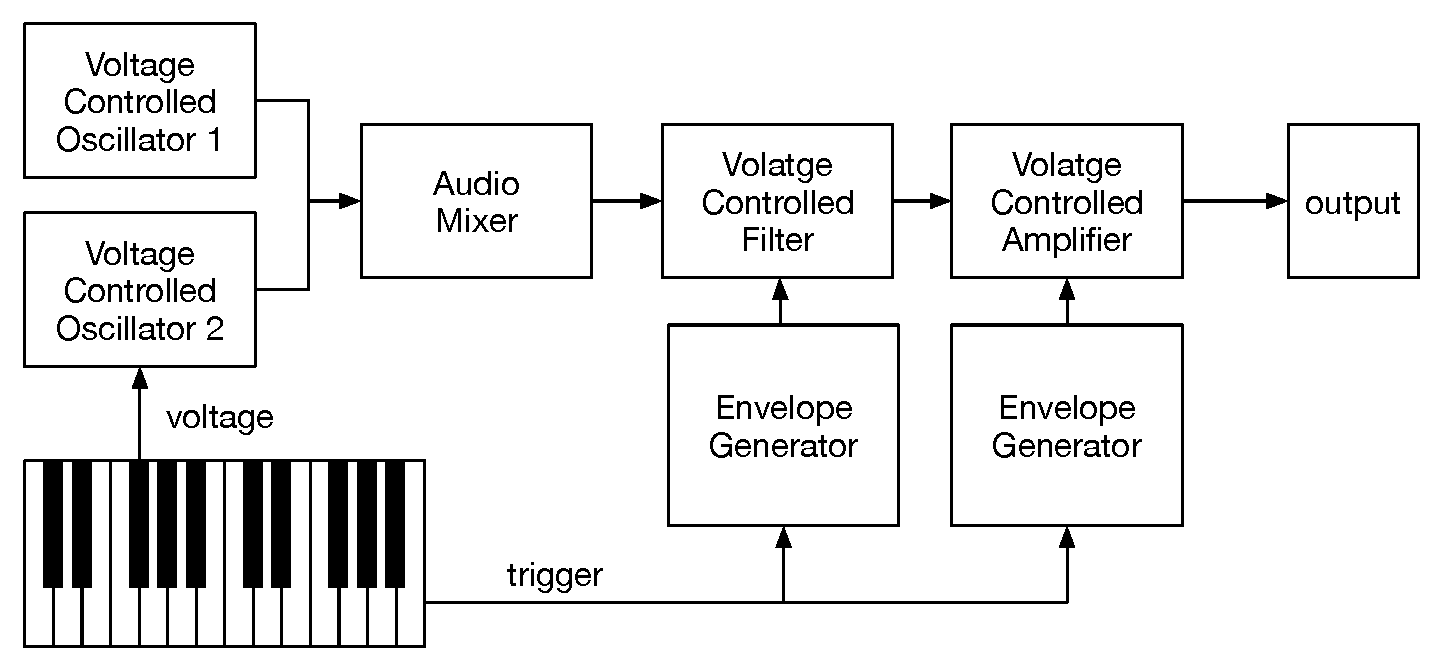
\includegraphics[width=\textwidth]{assets/synth_voice_block.pdf}
    \caption{Block Diagram of a Subtractive Synthesis Voice}
    \label{fig:synth_voice_block}
\end{figure}

The voltage controlled oscillators generate simple waveforms at the pitch coresponding to the note played on the keyboard. The user can typically choose between some combination of sawtooth, squareware, or triangle waveforms. The frequencies or timbre of the waveforms can then be modulated by the following filter and amplitude blocks.

One's first impression might be that modeling the oscillator would be simple. A digitally generated squarewave or sawtooth waveform should be trivial to implement. The 5kHz sawtooch waveform for example, would have a period of 8.82 samples when generated in a 44.1kHz audio environment. So the waveform would increase linearly from -1.0 to 1.0 over a length of 8.82 samples, then jump back to -1.0 and cycle through again. What does 0.82 sample mean in a discreet digital system? Figure~\ref{fig:aliasing_sawtooth} illustrates the problem with a trivial implementation. The left column shows a portion of an idealized 5kHz sawtooth waveform and the coresponding frequency content. Above the 5kHz fundamental frequency are harmonics that will be audible well beyond 100kHz. The right column shows the same portion of a 5khz sawtooth waveform in a 44.1kHz environment. The waveform itself is distorted and the higher harmonics are visible reflected back from the 22.05kHz nyquist limit.

\begin{figure}[H]
    \centering
    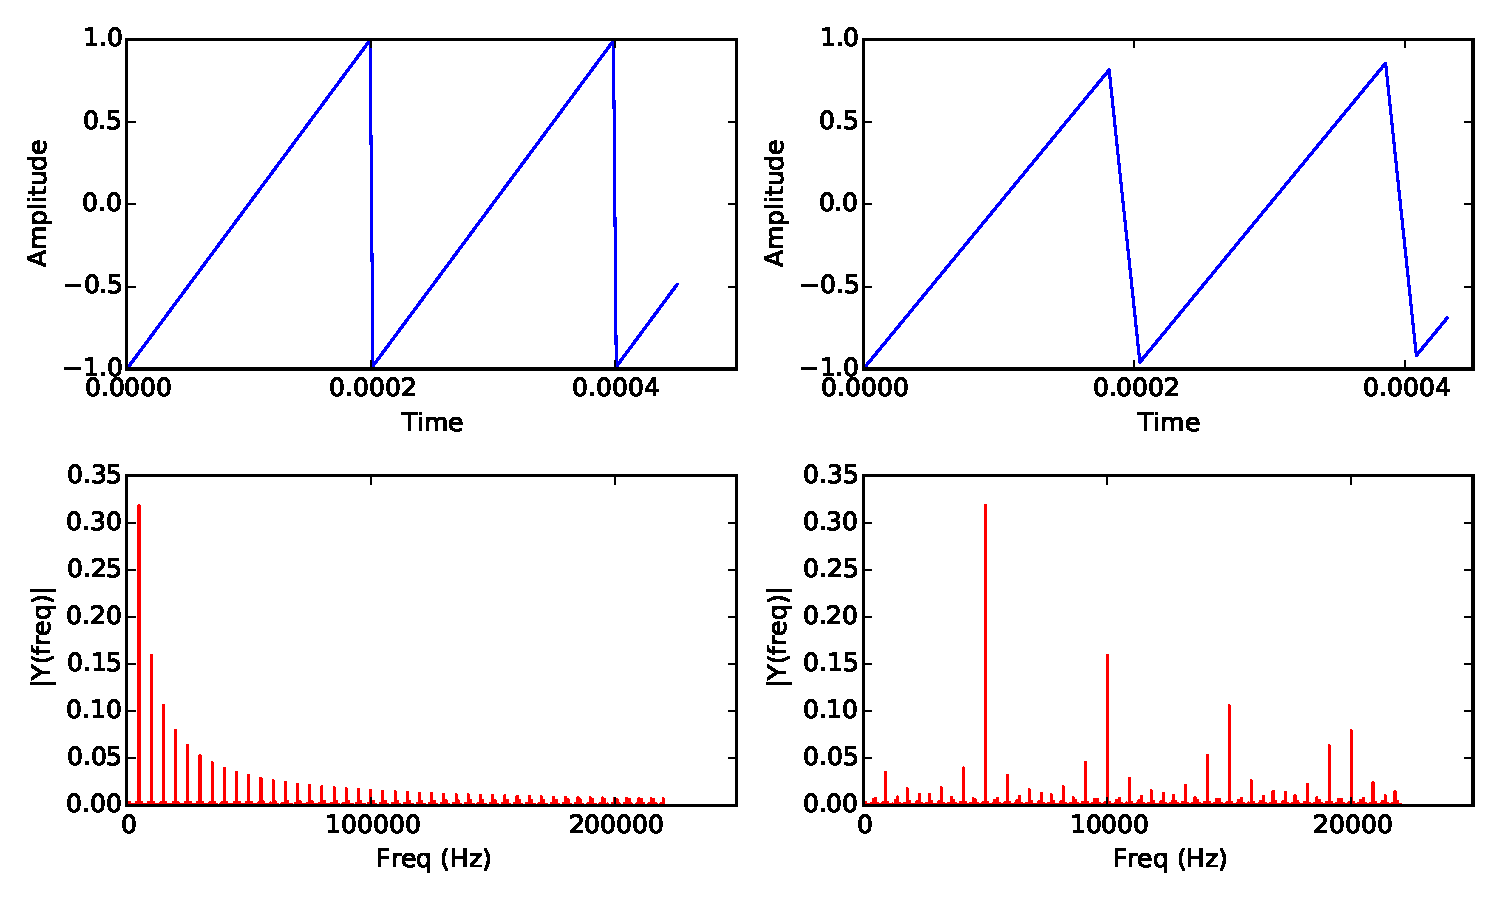
\includegraphics[width=\textwidth]{plots/graphics/sawtooth.pdf}
    \caption{Ideal and Aliased 5kHz Sawtooth waveform}
    \label{fig:aliasing_sawtooth}
\end{figure}

There are various methods to eliminate or reduce aliasing. The most effective is to generate the harmonics using a series of sin waves up to the nyquist limit or half of the system's sampling rate, but this also very processing intensive. Other less CPU intensive strategies involve using oversampling, bandlimiting, or other alias-supressing methods\cite{virtual_analog_synthesis}.

Evaluating and testing various strategies for alias reduction is beyond the scope of this project. But might be
interesting for follow up projects expanding on the material here.



\chapter{Anforderungsanalyse}
\section{General Application Requirements}

The Application has two components, the audio plugin hosted on the main CPU machine, and the processing node which runs on a networked SoC device. The audio plugin forwards midi control and audio data to the processing nodes. The nodes stream the processed audio data back to the audio plugin, which in turn streams it back to the host audio application. The total round-trip time, including processing, should not exceed 10ms. This is the maxium allowed latency for live sound applications. \cite{AES67-2013}

The applications must be self contained and work without the user needing to install any system libraries, frameworks or servers.\footnote{The only exception might be ZeroConf/Bonjour on Linux or Windows. See Appendix}

\subsection{Audio Plugin}

The audio plugin has the following requirements:

\begin{itemize}

\item runnable as a VST plugin in a standard audio application
\item locate and connect with one or processing nodes on the network
\item forward midi and audio data from the host audio application to the networked nodes
\item receives audio data from the networked nodes and streams this back to the host application

\end{itemize}

\subsection{Processing Node}

The processing node has the following requirements:
\begin{itemize}

\item broadcasts its availability and location on the network
\item accepts session initiated by the audio plugin
\item accepts controll data from the audio plugin
\item processes incoming audio data and midi data from the audio plugin
\item streams audio and midi data back to the audio plugin or to the next node in the processing chain

\end{itemize}




\chapter{Implementation}
\section{Architektur}

\section{Developement Environment}

\section{Networking Components}

These are general C++ components that are used in both the audio plugin and the processing nodes. They encapsulate the network communicatation handling.

\subsection{Socket Monitor}

The socket monitor class uses a posix select() function to montitor the status of a collection of socket file descriptors. When a file descriptor becomes ready to read from or write to the socket monitor can notify a registered delegate class via a specified callback.

\begin{itemize}

\item runs as a thread, blocks on select() until one of the managed filedescriptors becomes ready to read then notifies corresponding listener

\item define abstract listener class: FileDescriptorListener
\item select can be configured with a timeout, unblocking the call, inorder to check status of application ( everything ok? should i shut down? should i update? etc.. ) but it is more effiecient to use a control socket that can be trigged by the app to unblock the select call when needed.
\item


\end{itemize}

\subsection{ZeroConf Manager}

The ZeroConf Manager class encapsulates calls to the system's bonjour/zeroconf deamon.

\subsection{AudioStream Manager}

This class is responsible for streaming audio data to or from a specified udp port. It implements

\chapter{Conclusion}
conclusion

\bibliography{references}{}
\bibliographystyle{plain}

\chapter{Appendix A}
\section{Compiling the Source Code}

Download the Juce C++ Library from GitHub

https://github.com/julianstorer/JUCE

Additionally download and install the DrowAudio Juce Module Extensions

https://github.com/drowaudio/drowaudio.git
\section{Bonjour}

Instructions for installing bonjour:

\end{document}